\section{问题二模型的建立与求解}

问题二在问题一的基础上放松了确定性假设。每天的电价曲线相同且完全已知，不确定性全部来自负载与光伏功率的逐时段变化。微网向外的供电不得低于小区负载，一旦不足，缺口部分必须以交易时刻电价的 $5$ 倍紧急购电；除紧急购电费用以外，其余时段的购电费用一律按计划购电量结算，与计划电量是否被实际使用无关。

问题一假设电价与负载逐时段已知，唯一的不确定来源是光伏预测偏差，模型可退化为确定性的单日线性规划；问题二把不确定性整体搬到负载侧与光伏侧，0:00 制定计划时当天的负载曲线与光伏曲线尚未揭晓，决策只能依据此前的历史数据，不得引入任何前视信息。微网向外的供电不得低于小区负载，计划不足的部分必须以 $5$ 倍电价紧急购入，计划偏多的部分只能存入储能或弃置，两类偏差的代价明显不对称。单看一个时段，这一取舍具有\textbf{报童问题}的结构，但储能状态在日内 $144$ 个时段之间连续递推，需要刻画的并非各时段彼此独立的不确定性，而是整条净负荷曲线的联合变化，因此本文把问题形式化为带储能跨时段耦合的\textbf{两阶段随机线性规划}：计划购电量在 0:00 一次确定，对所有可能的次日情形取同一值；储能充放电、紧急购电与弃置电量则随当天揭晓的实际曲线调整。问题的难点在于次日净负荷的联合分布未知，只能由有限的历史数据推断，本文以历史日的完整曲线作为情景、以经验期望近似真实期望，情景的选取范围、采样单位与前视约束则一并由数据自身的月度差异、周周期与残差相关性决定。

\subsection{数据预处理与探索性分析}

\subsubsection{结构性证据}

情景池的构造依据来自四方面的数据事实。其一是\textbf{月度差异}：负载与光伏的月度变化不同步，净负荷起伏更明显，5 月与 12 月的月均日累计净负荷分别为 $38.28$ MWh/d 与 $76.26$ MWh/d，后者约为前者的 $1.99$ 倍，代表月份的日内净负荷都呈午间下降、傍晚回升，午间低谷的深度差别很大，全年样本不宜混合，应优先取与决策日季节相近的日期。其二是负载的\textbf{周周期}：先减去各时段的全年均值，再算相隔 $1$ 至 $14$ 天的同刻相关系数，滞后 $7$ 天与 $14$ 天分别达到 $0.9722$ 与 $0.9600$，明显高于邻近滞后（见图~\ref{fig:eda-weekly-lag}），说明上周同一时段的观测更可能保留相似规律。其三是预测误差的\textbf{日内延续性}：以负载上周同刻值与光伏过去 $7$ 日同刻均值构成的组合基线剥离可预测成分后，相邻 $10$ 分钟净负荷残差的相关系数仍有 $0.8497$，情景因此以完整日曲线为采样单位。\textbf{星期几}是第四个来源，可解释去均值后方差的 $85.28\%$；日总电量最低的两天是周五与周六，约 $78.3$ 与 $78.4$ MWh，其余五天约 $123.9$ 至 $124.1$ MWh，相差约 $1.58$ 倍，这否定了把周六与周日同划为周末的假设，因为周日是高负载日。

\begin{figure}[htbp]
\centering
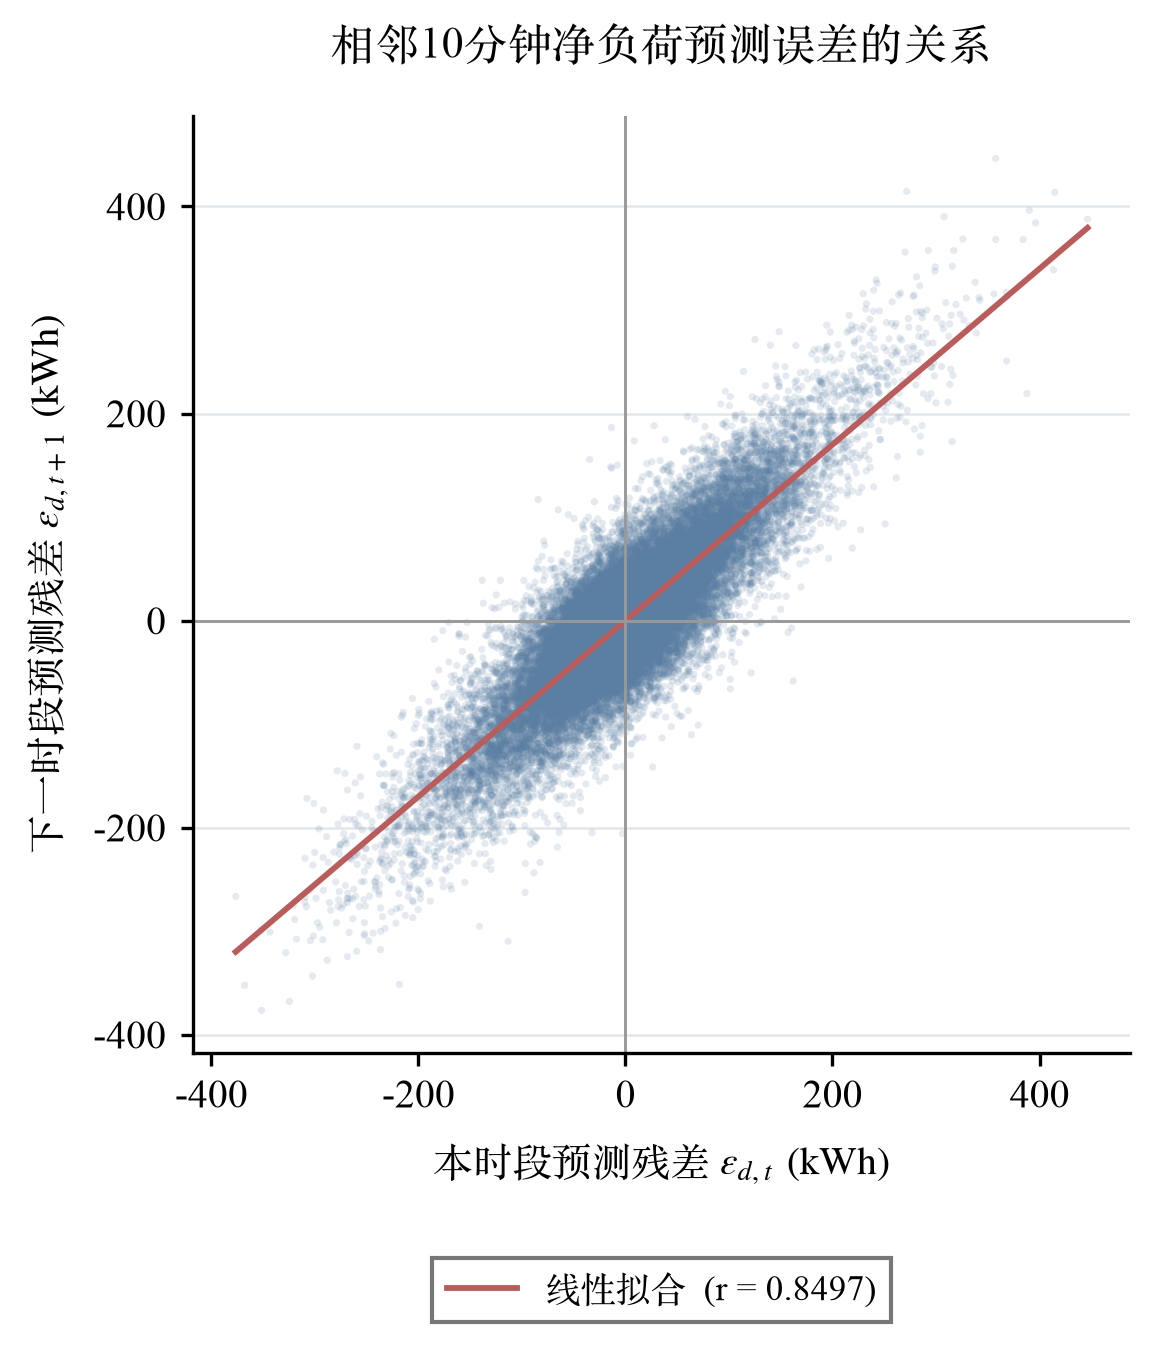
\includegraphics[width=0.45\textwidth]{figures/010_residual.png}
\caption{相邻 10 分钟净负荷预测误差的关系}
\label{fig:residual}
\end{figure}

图~\ref{fig:residual} 显示相邻时段的净负荷预测误差之间存在明显的正相关：上一时段偏高的误差倾向于延续到下一时段，与相邻 $10$ 分钟残差相关系数 $0.8497$ 的定量结果一致。这意味着净负荷的不可解释成分并非逐时段独立，若在情景生成时对时段独立抽样，将丢失这一日内惯性，从而低估整条净负荷曲线的波动幅度；因此本文以完整历史日曲线作为情景单位，逐日整段抽取，保留时序相关性。

\subsubsection{特征集合与核权重}

最终处境由季节圆周位置、上周同日净负荷、前三日光伏均值、上周同日负载、前七日净负荷均值与低负载日标志构成，特征集合为 \texttt{season}、\texttt{net\_lag\_7d}、\texttt{pv\_mean\_3d}、\texttt{load\_lag\_7d}、\texttt{net\_mean\_7d} 与 \texttt{low\_load\_day}。以 $\boldsymbol z_d$ 与 $\boldsymbol z_\omega$ 表示验证日与情景日的标准化处境向量，核权重取高斯形式
\begin{equation}
\pi_{d,\omega}=
\frac{\exp\left[-\|\boldsymbol z_d-\boldsymbol z_\omega\|_2^2/(2h^2)\right]}
{\sum_{j\in\Omega_d}\exp\left[-\|\boldsymbol z_d-\boldsymbol z_j\|_2^2/(2h^2)\right]},\label{eq:kernel}
\end{equation}
其中 $\|\boldsymbol z_d-\boldsymbol z_\omega\|_2$ 是标准化处境距离，$h$ 为带宽，控制权重衰减的快慢。带宽以\textbf{平均能量分数}唯一选优，冻结取值为 $h=1.043841$。评分同样采用平均能量分数，以 $\boldsymbol x_\omega$ 与 $\boldsymbol y_d$ 表示两日的 $144$ 维净负荷曲线，定义
\begin{equation}
ES_d=\sum_{\omega\in\Omega_d}\pi_{d,\omega}\|\boldsymbol x_\omega-\boldsymbol y_d\|_2
-\frac12\sum_{\omega,\omega'\in\Omega_d}\pi_{d,\omega}\pi_{d,\omega'}\|\boldsymbol x_\omega-\boldsymbol x_{\omega'}\|_2,\label{eq:es}
\end{equation}
其中第一项度量情景曲线到真值的加权距离，第二项是情景间的加权分散度并从分数中扣除；分数越小越好。特征筛选与带宽搜索的完整过程详见附录 D。

\subsubsection{赋权方案的采用依据}

全年 $334$ 天的平均能量分数为：等权基线 $1334.486$ kW，旧特征集 $1248.040$ kW，修订特征集 $551.071$ kW。修订方案相对等权基线改善 $58.706\%$，改善日数 $328/334$；相对旧特征集改善 $55.845\%$，改善日数 $318/334$，两者均超过预设的 $3\%$ 采纳门槛。核加权同时提高了权重集中程度，有效情景数 $K_{\mathrm{eff}}$ 的均值为 $12.17$，范围为 $1.01$ 至 $40.08$。为排除评分口径造成的假象，另做决策层抽样回测兜底：每月取前 $2$ 天共 $22$ 天，三套权重分别求解决策层与执行层并在真实曲线上结算，修订特征集的总费用为 $1{,}125{,}932.8$ 元，比等权基线低 $10.354\%$。

\subsection{模型建立}

\subsubsection{模型假设}

\begin{enumerate}
\item \textbf{跨日近视}：储能的跨日影响有限，即将储能电量留到第二日消耗的边际回报处处不超过今日释放的即时收益。该假设的口头论证(见附录)在当前模型族内不可检验，本工作把它改写为待检验命题，并在同一情景池、同一核权重、同一执行层下用含终端价值的远视模型做配对对照，检验设计与结论见后文。
\item \textbf{已购电量可以弃置}：计划购电按量结算、无需用尽，允许 $W_{d,t}^{\omega}>0$。
\item \textbf{紧急购电不进储能}：紧急购电只用于补足负载缺口，不作为储能充电的来源。该性质不能由 $5P_t>P_t$ 自动保证，因为跨时段被比较的是低价时段的 $5P_t$ 与高价时段的 $5P_{t'}$，储能让两者之间的套利成立；又因充电量是情景特定变量而计划购电量是全情景共享变量，模型有动机用情景内的廉价紧急电充电替代提高共享计划。本模型因此把它写成显式的线性约束，即形式化建模中的充电来源约束。
\item \textbf{购电无功率上限}：题面未对计划购电与紧急购电设置功率限制，模型不设。
\item \textbf{情景代表性}：次日与 $\mathcal{H}_d$ 中同季节历史日近似可交换，$\Omega_d$ 的经验分布可作为次日净负荷条件分布的近似。
\end{enumerate}

\subsubsection{形式化建模}

\textbf{情景生成。} 对每个 $d\in\mathcal{D}$，在 0:00 从候选历史池 $\mathcal{H}_d$ 中以整天为单位抽取情景并按数据预处理一节得到的核函数赋权，得到 $\Omega_d$ 与 $\pi_{d,\omega}$。每个情景 $\omega$ 直接提供历史日 $\omega$ 的完整实测曲线。由于 $\mathcal{H}_d$ 只含 $j<d$ 的历史日，情景集合及其权重不含任何未来信息。整日抽取的好处是历史日天然保存了日内的时序结构，不需要额外假定残差的分布形式。

\textbf{决策变量。} 第一阶段变量为计划购电量 $G_{d,t}\ge0$ 与其中划给储能充电的份额 $G^{\mathrm{c}}_{d,t}$，二者在 0:00 一次性确定并对所有情景取同一值；第二阶段变量为逐情景的储能充放电量、储电量、紧急购电量与弃置电量，在情形揭晓后确定。

\textbf{目标函数。} 计划购电量在 0:00 定死，紧急购电量随次日实际曲线浮动，模型要在确定发生的计划电费与期望的紧急购电费之间取舍：
\begin{equation}
\min \;\; \sum_{t \in \mathcal{T}} P_t\, G_{d,t} \;+\; \sum_{\omega \in \Omega_d} \pi_{d,\omega} \sum_{t \in \mathcal{T}} 5\, P_t\, E_{d,t}^{\omega}
\;+\;\varepsilon\sum_{\omega\in\Omega_d}\pi_{d,\omega}\sum_{t\in\mathcal{T}}\bigl(C_{d,t}^{\omega}+D_{d,t}^{\omega}\bigr).\label{eq:obj2}
\end{equation}
其中 $P_tG_{d,t}$ 是按附件 1 电价结算且确定发生的计划购电费；$5P_tE^{\omega}_{d,t}$ 是情景 $\omega$ 下的紧急购电费，单位缺货成本相当于 $4P_t$；权重归一，第二项即次日紧急购电费的期望估计；$\varepsilon=10^{-6}$ 元/kWh 是去退化项，只用于在等价的充放电路径中挑出动作最少的一条，不改变计划购电量与主成本。目标函数只覆盖当天，不含日末储能对次日的价值，这是跨日近视假设在模型中的落点。两项系数的差异决定了计划的保守程度：过剩只付 $P_t$，缺货却要付 $5P_t$，因此把计划量从均值向上推到净负荷分布的 $0.8$ 分位数是有利的；储能项在此的作用是把低价时段的富余电量搬到高价时段，它自身不改变这一分位数结构的定性结论。第二项把 $144$ 维的不确定性压缩为一个标量，使第一阶段决策可以在不知道具体情形的前提下作出。

\textbf{能量平衡约束。} 每个时段的电能来源与去向必须相等：
\begin{equation}
G_{d,t} + E_{d,t}^{\omega} + R_{d,t}^{\omega} + D_{d,t}^{\omega} = L_{d,t}^{\omega} + C_{d,t}^{\omega} + W_{d,t}^{\omega}, \qquad \forall \omega \in \Omega_d,\ t \in \mathcal{T}.\label{eq:balance2}
\end{equation}
其中 $G_{d,t}$ 与 $E^{\omega}_{d,t}$ 是外购电量，$R^{\omega}_{d,t}$ 是情景光伏，$D^{\omega}_{d,t}$ 是储能放电；$L^{\omega}_{d,t}$ 是情景负载，$C^{\omega}_{d,t}$ 是储能充电，$W^{\omega}_{d,t}$ 是弃置电量，弃光与已购未利用合并计入后者。弃置变量显式出现在去向一侧，使计划购电量可以多于当日实际所需，模型不必把多余的计划电强行塞进储能。该约束对每个情景逐时段成立，是后续全部约束的共同基础。等式两侧都是原始物理量，未经任何线性化处理。

\textbf{储能递推与共同出发点。} 储能状态在时段之间递推，充电按 $\eta_c$ 折算入库，放电按 $\eta_d$ 折算出库：
\begin{equation}
S_{d,t+1}^{\omega} = S_{d,t}^{\omega} + \eta_c\, C_{d,t}^{\omega} - \frac{D_{d,t}^{\omega}}{\eta_d}, \qquad
S_{d,1}^{\omega} = S_{d,1}, \qquad \forall \omega \in \Omega_d,\ t \in \mathcal{T}.\label{eq:soc2}
\end{equation}
其中 $S^{\omega}_{d,t}$ 是情景 $\omega$ 下时段 $t$ 开始时的储电量，$\eta_c=\eta_d=0.9$ 使单程损耗为 $10\%$、往返损耗为 $19\%$。第二式是共同出发点约束，所有情景从 0:00 实测的同一储能状态出发。它的作用是把情景差异限制在负载与光伏两类外生曲线上：若允许各情景自由选择起始储电量，模型就能用起点差异掩盖计划购电量的不足，非预期性约束会被架空。递推式在情景之间彼此独立，唯一的耦合来自第一阶段变量与共同出发点。

\textbf{储能边界、充放电功率与非负性。} 储电量、充放电动作与购弃电量都必须落在设备与题设允许的范围内：
\begin{equation}
S^{\min} \le S_{d,t}^{\omega} \le S^{\max}, \quad \forall t \in \mathcal{T}^+; \qquad
0 \le C_{d,t}^{\omega}, D_{d,t}^{\omega} \le \bar{e}, \quad \forall t \in \mathcal{T}; \qquad
G_{d,t},\ E_{d,t}^{\omega},\ W_{d,t}^{\omega} \ge 0,\label{eq:bound2}
\end{equation}
以上约束对所有 $\omega \in \Omega_d$ 成立。其中 $S^{\min}=1200$ kWh 与 $S^{\max}=10800$ kWh 是储电量上下限，$\bar e\approx833.33$ kWh 是单时段最大充放电能量。三组界分别防止储能过充过放、限制充放电功率在额定值以内、保证购电量与弃置量非负。储能动作因此只能在 $1200$ 至 $10800$ kWh 的电量区间与 $833.33$ kWh 的时段功率预算内开展，后文出现的日末储电量停在下限这一现象并非边界所迫，而是目标函数的选择。

\textbf{充电来源约束。} 为防止模型用情景内的紧急购电给储能充电，充电能力必须与全情景共享的第一阶段变量绑定：
\begin{equation}
0 \le G^{\mathrm{c}}_{d,t} \le G_{d,t} - \Delta_{d,t}, \qquad
C_{d,t}^{\omega} \le \max\bigl(0,\ R_{d,t}^{\omega} - L_{d,t}^{\omega}\bigr) + G^{\mathrm{c}}_{d,t},
\qquad \forall \omega \in \Omega_d,\ t \in \mathcal{T}.\label{eq:charge2}
\end{equation}
其中 $G^{\mathrm{c}}_{d,t}$ 是计划购电量中划给储能充电的份额，第一式把它的上限取为扣除期望净负荷缺口 $\Delta_{d,t}=\sum_\omega\pi_{d,\omega}\max(0,L^{\omega}_{d,t}-R^{\omega}_{d,t})$ 之后的余额，即计划电先留给负载；第二式规定充电只能来自该情景该时段的光伏富余与这份共享份额之和。若不加这两条，模型会出现套利：低价时段的 $5P_t$ 低于高价时段的 $5P_{t'}$，用情景内的紧急电充电再到高峰放电替代紧急购电有利可图，全年 $365$ 天中有 $103$ 天出现该行为。这两条是充电侧唯一的来源限制，放电侧不受此限，因为放电只减少储能存量，不引入新的外购电量。

\textbf{执行层。} 决策层输出计划购电量之后，白天的实测曲线揭晓，需要按实际数据确定补救动作：
\begin{align}
\min &\sum_{t \in \mathcal{T}} \Bigl(5 P_t E_{d,t} + \varepsilon\,(C_{d,t}+D_{d,t})\Bigr) \notag\\
\text{s.t.}\quad & C_{d,t} \le \max\bigl(0,\ R_{d,t}+G_{d,t}-L_{d,t}\bigr), \notag\\
& E_{d,t} \le \max\bigl(0,\ L_{d,t}-R_{d,t}-G_{d,t}\bigr).\label{eq:exec2}
\end{align}
其中 $A_{d,t}=R_{d,t}+G_{d,t}-L_{d,t}$ 是扣除负载之后的可用电量，充电上界取其正部，紧急购电上界取其负部。执行层的 $G_{d,t}$ 是已知常数，缺口时段迫使 $C_{d,t}=0$，富余时段迫使 $E_{d,t}=0$，因此不存在一边紧急购电一边充电的时段，该结论精确成立。该互斥性是负载优先的直接推论：先满足负载，再用余量充电，两者不可能同时为正。求解该问题得到实际执行路径，也就是结果文件中充放电量与紧急购电量两张工作表的数值来源，其中 $E_{d,t}>0$ 的时段与购电量按表 3 格式填报。执行层与决策层的区别在于它使用实测曲线，因此求解结果是唯一的实际路径，不再带有情景维度。

\textbf{跨日链与全年结算。} 储能在相邻两日之间链式衔接，$S_{d+1,1}=S_{d,145}$，2025-01-01 的起点日初储电量取 $6000$ kWh；1 月作为冷启动期滚动储能状态但不输出结果。全年官方结算费用为
\begin{equation}
C_{\mathrm{official}} = \sum_{d \in \mathcal{D}_{\mathrm{out}}} \sum_{t \in \mathcal{T}} \left( P_t\, G_{d,t} + 5\, P_t\, E_{d,t} \right),\label{eq:official2}
\end{equation}
其中 $G_{d,t}$ 与 $E_{d,t}$ 都是实际执行路径上的量，求和范围为输出日期集合与全部 $144$ 个时段。该口径只含真实发生的计划购电费与紧急购电费，是全文比较各方案费用的统一尺度。

\subsubsection{跨日近视假设的检验设计}

跨日近视直接决定日末储电量与弃置电量的水平，本文把它改写为可判定的命题并按事先固定的口径补做检验，论证史见附录 A 至附录 C。

原口头论证的承重环节是一条充分条件：终端价值函数切线斜率的最大绝对值不超过晚高峰电价的最小值。该条件在当前模型族内不可检验，因为其左端所引用的量只在含终端价值的模型中才有定义，近视模型内没有任何最优性条件涉及它。否证的对象因此不是跨日近视近似不准这一数值判断，而是该论证构成对跨日近视假设的检验这一方法论主张，该结论只依赖模型结构，与具体数据无关。

由于充分条件不可检验，本文补做远视对照：在目标函数中恢复终端价值项，并用分段线性下界从下方支撑终端价值函数，记 $\theta^{\omega}_{d}$ 为情景 $\omega$ 下的终端价值辅助变量，$a_{d,q}$ 与 $b_{d,q}$ 为第 $q$ 条切线的斜率与截距，则终端价值以
\begin{equation}
\theta^{\omega}_{d} \;\ge\; a_{d,q}\, S^{\omega}_{d,145} + b_{d,q},
\qquad q = 0,\ldots,Q_d-1,\quad \forall \omega \in \Omega_d\label{eq:terminal2}
\end{equation}
自下方被支撑。配对对照在同一情景池、同一核权重与逐元素相同的执行层下进行，远视模型的全年官方结算费用为 $17{,}036{,}556.63$ 元，比近视基线高 $38{,}051$ 元，相对 $-0.2233\%$，未达事先固定的 $0.5\%$ 采纳阈值，因此保留近视模型。该负结果只在决策层远视而执行层近视这一具体口径下成立，既不构成对跨日近视假设的证明，也不回答跨日近视究竟有多大代价，完整的配对数据与适用边界见附录 C。

\subsection{模型求解}

求解按三步推进，三步的先后关系固定。

\textbf{第一步，决策层。} 对每一天，用当日候选历史池与冻结的核权重求解两阶段随机线性规划，得到全时段计划购电量 $G_{d,t}$。该步输入只含 $j<d$ 的历史日，不含当日及以后的任何观测。

\textbf{第二步，执行层。} 白天的实测负载与光伏揭晓后，固定第一步给出的 $G_{d,t}$，把实测曲线代入补救问题求解，得到实际执行路径 $C_{d,t},D_{d,t},S_{d,t},E_{d,t},W_{d,t}$，也就是结果文件中充放电量与紧急购电量两张工作表的数值来源。

\textbf{第三步，跨日链。} 令 $S_{d+1,1}=S_{d,145}$ 把日末储电量传递到次日，再回到第一步推进下一天，构成滚动时域（rolling horizon）决策链。滚动自 2025-01-01 的 $6000$ kWh 初始储电量开始，1 月作为冷启动期只推进储能状态、不输出结果，因此 2 月 1 日的日初储电量是滚动结果而非重置值。

\subsection{结果分析}

\subsubsection{模型验证}

全年 $365$ 天的求解结果全部通过能量平衡、储能递推、储能边界、充放电功率、充放电互斥、紧急购电与充电互斥、跨日链与费用重算等各项形式化断言，最大残差量级为 $10^{-13}$。\textbf{无前视泄漏}检验通过：把目标日及其之后的原始观测整体扰动后重建处境特征、候选池与核权重并重跑该日决策，候选池、权重与计划购电量逐元素完全不变，逐日决策输入不含任何未来信息。

一处需要如实记录的模型性质是\textbf{弃置电量}。全年弃置电量为 $3{,}848{,}719.1$ kWh，占计划购电量的 $17.61\%$，是全年充电量 $624{,}209.4$ kWh 的 $6.166$ 倍，$334$ 天中有 $333$ 天出现弃置，计划购电总量超出实际净负荷 $3{,}911{,}474.8$ kWh。该现象是报童式计划与跨日近视假设共同作用的结果：缺货成本 $4P_t$ 与过剩成本 $P_t$ 使最优计划落在净负荷分布的 $0.8$ 分位数上，多数日子的计划必然高于当日实际净负荷；又因跨日近视，日末储电量每天都在下限，当日用不掉的多余电量既不能留到次日，也不值得为当天并不存在的缺口充电，因为充电只增加往返损耗，于是计入弃置。该弃置在给定模型内是最优的，但它同时标出了跨日近视假设的代价上限，也是检验该假设时最值得复查的一项。该性质的完整复算见附录 A 与附录 C。

\subsubsection{敏感性分析}

\textbf{充放电效率口径。} 题面给出的充放电效率为 $90\%$，这允许两种读法：分别取充电效率与放电效率为 $0.9$，或取往返效率为 $0.9$ 从而单程效率为 $\sqrt{0.9}\approx0.9487$。本文采用前者，即 $\eta_c=\eta_d=0.9$，单程损耗 $10\%$、往返损耗 $19\%$。若改用后者，往返损耗由 $19\%$ 降到 $10\%$，储能的套利与削峰收益同步上升，储能动作的幅度会增大，但计划购电量与弃置电量的相对关系不变。

\textbf{核加权方案与带宽。} 三套赋权方案的排序在评分与费用两个口径下一致：平均能量分数分别为 $551.071$、$1248.040$ 与 $1334.486$ kW，修订方案相对等权基线改善 $58.706\%$；决策层抽样回测的总费用分别为 $1{,}125{,}932.8$、$1{,}203{,}114.1$ 与 $1{,}255{,}970.2$ 元，与评分排序相同。带宽在 $[0.05,20]$ 上经 $25$ 点粗搜与三轮 $17$ 点细搜共 $77$ 个候选唯一选优，得到内部最优 $h=1.043841$，未触及搜索边界，说明结论对赋权方案与带宽的选择不敏感。带宽搜索过程与三套方案的全部对比数据详见附录 D。

\textbf{有效情景数与情景覆盖。} 有效情景数 $K_{\mathrm{eff}}$ 的均值为 $12.17$，范围为 $1.01$ 至 $40.08$。权重集中会缩小情景覆盖并可能低估尾部风险，这是核加权方案的固有代价，本文以决策层抽样回测与形式化核验两条独立证据兜底：回测显示紧急购电量从 $39{,}212.5$ kWh 降到 $14{,}065.2$ kWh，说明收缩情景覆盖并未转化为尾部风险的上升。

\textbf{紧急购电的成因定位。} 全年 $70$ 天出现紧急购电，合计 $55{,}844.1$ kWh，占计划购电量的 $0.256\%$，单日紧急购电量的中位数为 $0$，最集中的两天是 2025-06-01 的 $9{,}646.9$ kWh 与 2025-06-02 的 $8{,}003.5$ kWh。成因是 5 月末连续两个低负载日之后，6 月负载出现约 $50\%$ 的季节跃升，超出了仅含 5 月的候选池所覆盖的范围。这说明紧急购电的触发条件是候选池的季节覆盖而非计划分位数本身，把池的月份环形距离设为 $1$ 是在季节跃升边界上付出的代价。

\subsubsection{结果与讨论}

\textbf{全年结果。} 2025-02-01 至 12-31 共 $334$ 天，计划购电总量 $21{,}850{,}664.3$ kWh、计划购电费 $16{,}814{,}531.4$ 元；紧急购电总量 $55{,}844.1$ kWh、紧急购电费 $183{,}974.3$ 元；官方结算费用合计 $16{,}998{,}505.7$ 元。$334$ 天中有 $70$ 天出现紧急购电，紧急购电量占计划购电量的 $0.256\%$。储能日末储电量恒为下限 $1200$ kWh，日初储电量因此也恒为 $1200$ kWh，全年日内储电量在 $1200$ 至 $6609.6171$ kWh 之间循环，从未触及上限。全年弃置电量 $3{,}848{,}719.1$ kWh，占计划购电量的 $17.61\%$。

\textbf{指定日期结果。} 下表按表 1 与表 2 的格式给出表 3 指定日期 2025.3.20、2025.6.21、2025.9.23 与 2025.12.21 的结果，随后按表 3 的格式给出紧急购电结果。全部数值与结果文件逐项一致。表 1 的时段标签照抄附件 5 模板，数据按位置对齐，即模板第 $k$ 个数据列对应附件第 $k$ 个观测；表 2 填报的是实际执行路径，不带情景上标。

\begin{table}[htbp]
\centering
\caption{微网在指定时间段的购电量及全天的购电量和购电费}
\label{tab:purchase2}
\begin{tabular}{lrrrr}
\toprule
时间段 & 2025.3.20 & 2025.6.21 & 2025.9.23 & 2025.12.21 \\
\midrule
10:00-10:10 & 52.3188 & 3.1956 & 1.4019 & 383.4853 \\
12:00-12:10 & 0.6003 & 0.0169 & 0.0000 & 146.4846 \\
14:00-14:10 & 15.7876 & 6.8903 & 1.2945 & 289.4603 \\
16:00-16:10 & 463.1452 & 118.6965 & 423.6913 & 760.4718 \\
18:00-18:10 & 709.3962 & 431.3985 & 761.1071 & 723.0931 \\
20:00-20:10 & 719.9573 & 627.2136 & 812.7410 & 723.1969 \\
全天购电量 & 70659.3527 & 44844.3573 & 67970.5973 & 90849.7502 \\
全天购电费 & 54644.6277 & 33288.6709 & 53225.9899 & 71365.2630 \\
\bottomrule
\end{tabular}
\end{table}

表中购电量单位为 kWh，购电费单位为元。全天购电费按计划购电量计算，即 $\sum_t P_tG_{d,t}$。四日的紧急购电量均为 $0$，故四日的官方结算费用与表~\ref{tab:purchase2} 的全天购电费相同。

\begin{table}[htbp]
\centering
\caption{储能设备在指定时间段的充放电量及 0:00 和 24:00 的储电量}
\label{tab:storage2}
\small
\setlength{\tabcolsep}{4pt}
\renewcommand{\arraystretch}{1.2}
\begin{tabular}{lcccc}
\toprule
时间段 & 2025.3.20 充电/放电 & 2025.6.21 充电/放电 & 2025.9.23 充电/放电 & 2025.12.21 充电/放电 \\
\midrule
0:00-4:00 & 46.9488 / 38.0285 & 170.7311 / 129.2618 & 1130.8873 / 20.4117 & 747.9330 / 52.6090 \\
4:00-8:00 & 62.6336 / 50.7332 & 67.1264 / 63.4028 & 180.2679 / 735.9268 & 1096.1437 / 157.6024 \\
8:00-12:00 & 30.6536 / 24.8294 & 0.0000 / 0.0000 & 6.0645 / 310.6095 & 107.4785 / 1310.7401 \\
12:00-16:00 & 344.5601 / 116.4673 & 0.0000 / 0.0000 & 2170.8368 / 859.2091 & 958.0034 / 630.3785 \\
16:00-20:00 & 192.5584 / 219.7624 & 97.0170 / 78.5838 & 111.8732 / 852.9341 & 94.3075 / 261.0590 \\
20:00-24:00 & 117.2726 / 193.8272 & 143.1059 / 115.9158 & 133.4679 / 244.9610 & 99.7832 / 101.5667 \\
0:00 储电量 & 1200.0000 & 1200.0000 & 1200.0000 & 1200.0000 \\
24:00 储电量 & 1200.0000 & 1200.0000 & 1200.0000 & 1200.0000 \\
\bottomrule
\end{tabular}
\end{table}

表中每个单元格的格式为充电量 / 放电量，电量单位为 kWh。四日的日内储电量区间分别为 $1200.0$ 至 $1510.1$、$1200.0$ 至 $1287.3$、$1200.0$ 至 $3148.6$、$1200.0$ 至 $2766.7$ kWh，全程落在 $[1200,10800]$ 内。

\begin{table}[htbp]
\centering
\caption{微网在指定日期的紧急购电量}
\label{tab:emergency2}
\small
\setlength{\tabcolsep}{5pt}
\renewcommand{\arraystretch}{1.2}
\begin{tabular}{cccccccc}
\toprule
\multicolumn{2}{c}{2025.3.20} & \multicolumn{2}{c}{2025.6.21} & \multicolumn{2}{c}{2025.9.23} & \multicolumn{2}{c}{2025.12.21} \\
\midrule
时间段 & 购电量 & 时间段 & 购电量 & 时间段 & 购电量 & 时间段 & 购电量 \\
\midrule
无 & 0 & 无 & 0 & 无 & 0 & 无 & 0 \\
\bottomrule
\end{tabular}
\end{table}

四日在优化计划下均未触发紧急购电。四日的实际净负荷分别为 $62{,}209.0$、$19{,}334.7$、$62{,}116.6$ 与 $89{,}037.8$ kWh，均不超过当日计划购电量 $70{,}659.4$、$44{,}844.4$、$67{,}970.6$ 与 $90{,}849.8$ kWh，因此 $E_{d,t}=0$ 对所有时段成立，表~\ref{tab:emergency2} 中相应填无。

\textbf{跨日近视假设的检验结论。} 支持该假设的口头论证（见附录）在当前模型族内不可检验，本工作把当年跳过的检验补做完整，并在同一情景池、同一核权重、同一执行层下做配对对照：远视模型的全年官方结算费用为 $17{,}036{,}556.63$ 元，比近视基线高 $38{,}051$ 元，相对 $-0.2233\%$，未达事先固定的 $0.5\%$ 采纳阈值，因此保留跨日近视假设与近视模型，负结果如实记录。这个负结果只在决策层远视而执行层近视这一配对口径下成立：它既不构成对跨日近视假设的证明，因为执行层的近视性是配对口径的一部分而非本次对照的发现，也不回答跨日近视究竟有多大代价。配对数据、负结果的传导机制与适用边界见附录 C。

